\chapter{Theoretical Framework}
\label{chap:theory}

\chapterquote{I am now convinced that theoretical physics is actually philosophy.}
{Max Born}

\section{Quantum Chromodynamics}
Quantum chromodynamics (\QCD) is the non-Abelian \SUgroup{3} gauge theory of the strong interaction.
Initially, it appears similar to \QED, with the single electric charge replaced by three conserved ``colour'' charges; there are, however, important differences between the two.

In the \QED Lagrangian, \EquationRef{eq:bg-theory:qed}, the electron carries one unit of charge, $-e$, the positron carries one unit of anti-charge $+e$ and the force is mediated by a massless photon~\cite{Martin:2009:Nuclear}.

\begin{gather}
  \Lagrangian_{\QED} = \bar{\psi} \left(i \gamma^{\mu}  \partial_{\mu} -m \right) \psi - e \bar{\psi} \gamma^{\mu} A_{ \mu} \psi - \frac{1}{4}F_{\mu\nu}F^{\mu\nu} 
  \intertext{where for a photon field $A_{\mu}$,}
  F_{\mu\nu} = \partial_{\mu} A_{\nu} - \partial_{\nu} A_{\mu} \nonumber
  \label{eq:bg-theory:qed}
\end{gather}


\subsection{QCD Compton Scattering and Boson-Gluon Fusion}
Here is an example of \texttt{feynmf} to produce Feynman diagrams.
The Makefile should be able to cope with them, but if not, to build \texttt{feynmf} files

\begin{itemize}
  \item run \texttt{make} once
  \item then run \texttt{mf \symbol{34}\textbackslash{}mode=localfont; input \$name\symbol{34}}
\end{itemize}

\begin{figure}[htpb]
  \centering
  \parbox{99.9mm}{
    \vspace*{5mm}
    \unitlength=1mm
    \begin{fmffile}{qcdcompton}
      \begin{fmfgraph*}(100,50)
         \fmfleft{iq,ip}
         \fmfright{og,oq}
         \fmf{photon,label=$\gamma (q)$}{ip,v1}
         \fmf{fermion,label=$q_1 (yp)$}{iq,v2}
         \fmf{fermion,label=$q (xp)$}{v2,v1}
         \fmf{fermion,label=$q_2$}{v1,oq}
         \fmf{gluon,label=$g$}{v2,og}
      \end{fmfgraph*}
    \end{fmffile}
    \vspace*{5mm}
  }
  \caption{\QCD Compton scattering (\yqgq).}
  \label{fig:bg-theory:qcdcompton}
\end{figure}

The \QCD Compton process (\FigureRef{fig:bg-theory:qcdcompton}), is not discussed in this section.

\section{Jet Algorithms}
\label{sec:bg-theory:jet_algorithms}
A comparison between different jet algorithms can be seen in \FigureRef{fig:bg-theory:jet_algorithms}.
This figure uses \texttt{eps} which is auto-converted to \texttt{pdf} when compiling.
Here the jets produced by \kt, \CA, \akt and SISCone are shown, using the same input distribution of particles and the same $R$-parameter in each case. 
The two highest \pT jets in the event, here shown in green and red, are essentially identical in each case, although the precise details of which particles are combined are different in each case.
Additionally, there is some variation in the ordering of the lower \pT jets.
The circular shapes of the \akt jets and the irregular outline of the \kt jets are particularly notable.

\begin{figure}[htpb]
  \centering
  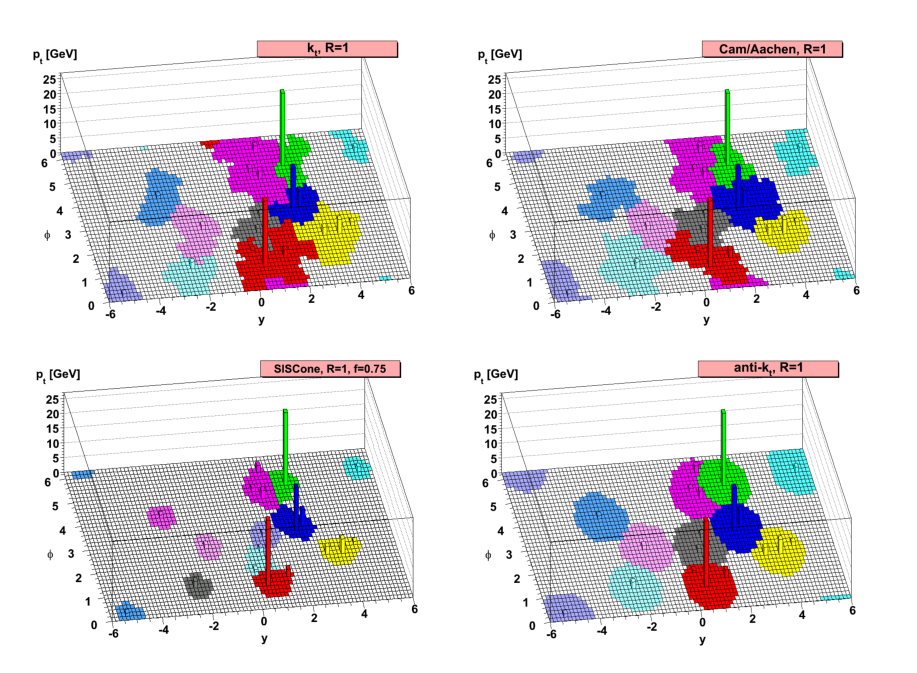
\includegraphics[width=\largefigwidth]{chapters/1.theory/JetAlgComparison.eps}
  \caption{A sample \Herwig generated parton level event, overlaid with random soft particles, clustered with four different jet algorithms, illustrating the shapes and sizes of the resulting hard jets. For \kt and \CA the detailed shapes are partially determined by the specific set of soft particles used, and would change if these were to be modified~\cite{Cacciari:2005:fastjet,Cacciari:2012:fastjet}.}
  \label{fig:bg-theory:jet_algorithms}
\end{figure}